\documentclass[aspectratio=169]{beamer}

\usetheme{Madrid}
\usecolortheme{seahorse}
\usepackage{listings}
\usepackage{tikz}
\usetikzlibrary{arrows.meta, shapes.geometric, positioning, fit, backgrounds}
\usepackage{booktabs}
\usepackage{xcolor}
\usepackage{graphicx}   % for \resizebox

% color palette
\definecolor{zblue}{RGB}{31, 78, 121}
\definecolor{zaccent}{RGB}{0, 112, 192}
\definecolor{zwarn}{RGB}{192, 80, 77}
\definecolor{zok}{RGB}{70, 130, 80}
\definecolor{zgray}{RGB}{89, 89, 89}
\definecolor{codebg}{RGB}{245, 246, 250}

\setbeamercolor{frametitle}{bg=zblue, fg=white}
\setbeamercolor{title}{bg=zblue, fg=white}
\setbeamercolor{structure}{fg=zaccent}
\setbeamercolor{block title}{bg=zblue!80, fg=white}
\setbeamercolor{block body}{bg=zblue!8}
\setbeamercolor{alerted text}{fg=zwarn}

% listings config
\lstdefinestyle{cpp}{
  language=C++,
  basicstyle=\ttfamily\scriptsize,
  keywordstyle=\bfseries\color{zblue},
  commentstyle=\itshape\color{zgray},
  stringstyle=\color{zok!80!black},
  backgroundcolor=\color{codebg},
  frame=single, framerule=0.4pt, rulecolor=\color{zaccent!40},
  xleftmargin=4pt, xrightmargin=4pt,
  breaklines=true, breakatwhitespace=false,
  tabsize=3, showstringspaces=false,
  morekeywords={NGuiKey, EPointName, EGuiReply, EDataLabel, EDataUnit,
                EDataRange, EPlotGroup, GuiFpn_t, ADataChannel,
                unique_ptr, unordered_map, make_unique, size_t,
                uint64_t, std}
}
\lstdefinestyle{python}{
  language=Python,
  basicstyle=\ttfamily\scriptsize,
  keywordstyle=\bfseries\color{zblue},
  commentstyle=\itshape\color{zgray},
  stringstyle=\color{zok!80!black},
  backgroundcolor=\color{codebg},
  frame=single, framerule=0.4pt, rulecolor=\color{zaccent!40},
  xleftmargin=4pt, xrightmargin=4pt,
  breaklines=true, showstringspaces=false, tabsize=4
}
\lstdefinestyle{json}{
  basicstyle=\ttfamily\scriptsize,
  keywordstyle=\color{zblue},
  stringstyle=\color{zok!80!black},
  backgroundcolor=\color{codebg},
  frame=single, framerule=0.4pt, rulecolor=\color{zaccent!40},
  xleftmargin=4pt, xrightmargin=4pt,
  breaklines=true, showstringspaces=false
}

\title{ZandrEA Write Path}
\subtitle{From HTTP POST to \texttt{ADataChannel}}
\author{}
\date{\today}

% ─────────────────────────────────────────────────────────────────────────────
\begin{document}

\begin{frame}
  \titlepage
\end{frame}

\begin{frame}{Roadmap}
  \tableofcontents
\end{frame}

% ─────────────────────────────────────────────────────────────────────────────
\section{Overview}

% Overview: two-row pipeline so it fits 16:9 width
\begin{frame}{30,000 ft view}

\begin{columns}[T]
\column{0.55\textwidth}

\resizebox{\linewidth}{!}{%
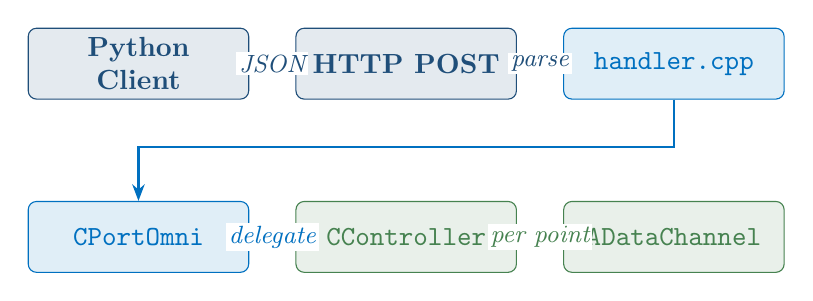
\begin{tikzpicture}[
  box/.style={rectangle, rounded corners=3pt, draw=#1, fill=#1!12,
              minimum width=2.8cm, minimum height=0.9cm, align=center,
              font=\normalsize\bfseries, text=#1},
  arr/.style={-{Stealth[length=6pt]}, thick, #1},
  lbl/.style={font=\small\itshape, midway, fill=white, inner sep=1pt}
]
% Row 1
\node[box=zblue]   (client)  at (0,0)   {Python\\Client};
\node[box=zblue]   (http)    at (3.4,0) {HTTP POST};
\node[box=zaccent] (handler) at (6.8,0) {\texttt{handler.cpp}};
% Row 2
\node[box=zaccent] (port)    at (0,-2.2)  {\texttt{CPortOmni}};
\node[box=zok]     (ctrlr)   at (3.4,-2.2){\texttt{CController}};
\node[box=zok]     (point)   at (6.8,-2.2){\texttt{ADataChannel}};

% Row 1 arrows
\draw[arr=zblue]   (client)  -- node[lbl]{JSON} (http);
\draw[arr=zblue]   (http)    -- node[lbl]{parse} (handler);
% Turn down
\draw[arr=zaccent] (handler.south) -- ++(0,-0.6) -| (port.north);
% Row 2 arrows
\draw[arr=zaccent] (port)   -- node[lbl]{delegate} (ctrlr);
\draw[arr=zok]     (ctrlr)  -- node[lbl]{per point} (point);
\end{tikzpicture}
}

\column{0.42\textwidth}
\vspace{1.2em}
Values arrive as a positional array. The server maps \texttt{values[i]} to
\texttt{ADataChannel} objects by index, using the order points were registered at construction.

\vspace{0.8em}
The client hard-codes the point list; there is no server-side name matching.
Both sides must agree on order \emph{a-priori}.
This can make it difficult to add future applications or points without breaking existing clients.
\end{columns}
\end{frame}

\begin{frame}{Complete Write-Path Sequence Diagram}

\begin{center}
\scalebox{0.62}{%
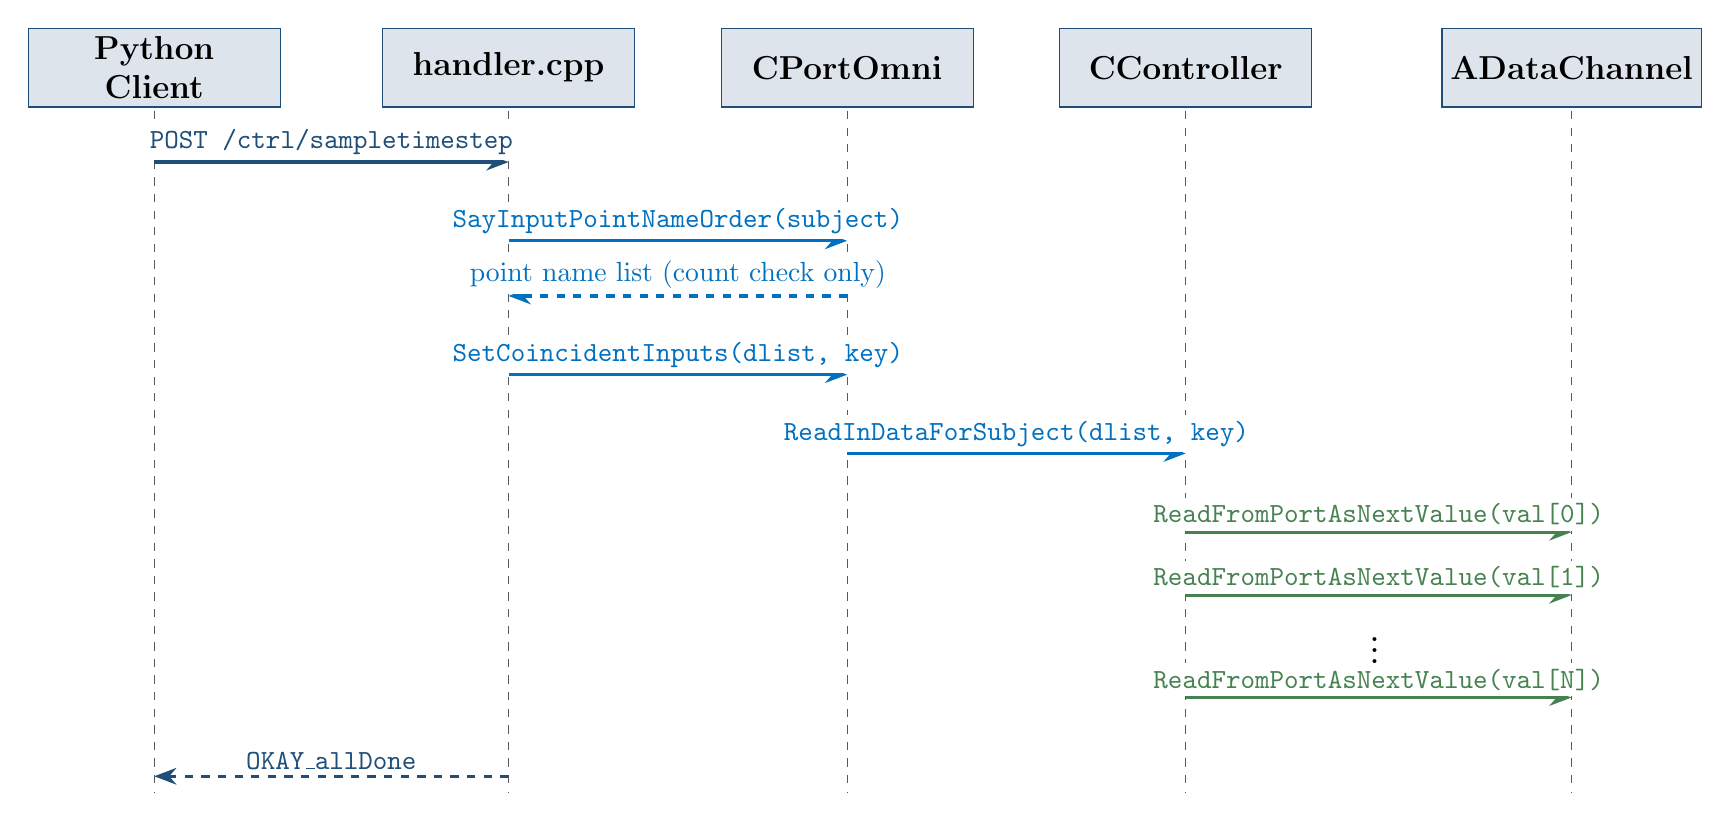
\begin{tikzpicture}[
  every node/.style={inner sep=3pt},
  actor/.style={rectangle, draw=zblue, fill=zblue!15,
                font=\large\bfseries,
                minimum width=3.2cm, minimum height=1.0cm, align=center},
  fwd/.style={-{Stealth[length=8pt]}, very thick, #1},
  ret/.style={-{Stealth[length=8pt]}, very thick, dashed, #1},
  lbl/.style={font=\normalsize, fill=white, inner sep=2pt}
]

% Actors
\node[actor] (py)  at (0,0)    {Python\\Client};
\node[actor] (hnd) at (4.5,0)  {handler.cpp};
\node[actor] (prt) at (8.8,0)  {CPortOmni};
\node[actor] (ctl) at (13.1,0) {CController};
\node[actor] (pt)  at (18,0)   {ADataChannel};

% Lifelines
\draw[draw=zgray, dashed] (0,-0.55)    -- (0,-9.2);
\draw[draw=zgray, dashed] (4.5,-0.55)  -- (4.5,-9.2);
\draw[draw=zgray, dashed] (8.8,-0.55)  -- (8.8,-9.2);
\draw[draw=zgray, dashed] (13.1,-0.55) -- (13.1,-9.2);
\draw[draw=zgray, dashed] (18,-0.55)   -- (18,-9.2);

% Messages
\draw[fwd=zblue]   (0,-1.2)  --
  node[lbl,above]{\texttt{POST /ctrl/sampletimestep}} (4.5,-1.2);

\draw[fwd=zaccent] (4.5,-2.2)  --
  node[lbl,above]{\texttt{SayInputPointNameOrder(subject)}} (8.8,-2.2);
\draw[ret=zaccent] (8.8,-2.9) --
  node[lbl,above]{point name list (count check only)} (4.5,-2.9);

\draw[fwd=zaccent] (4.5,-3.9)  --
  node[lbl,above]{\texttt{SetCoincidentInputs(dlist, key)}} (8.8,-3.9);

\draw[fwd=zaccent] (8.8,-4.9) --
  node[lbl,above]{\texttt{ReadInDataForSubject(dlist, key)}} (13.1,-4.9);

\draw[fwd=zok]     (13.1,-5.9) --
  node[lbl,above]{\texttt{ReadFromPortAsNextValue(val[0])}} (18,-5.9);
\draw[fwd=zok]     (13.1,-6.7) --
  node[lbl,above]{\texttt{ReadFromPortAsNextValue(val[1])}} (18,-6.7);
\node[font=\LARGE] at (15.5,-7.3) {$\vdots$};
\draw[fwd=zok]     (13.1,-8.0) --
  node[lbl,above]{\texttt{ReadFromPortAsNextValue(val[N])}} (18,-8.0);

\draw[ret=zblue]   (4.5,-9.0) --
  node[lbl,above]{\texttt{OKAY\_allDone}} (0,-9.0);

\end{tikzpicture}
}
\end{center}
\end{frame}

% ─────────────────────────────────────────────────────────────────────────────
\section{Client Side}

\begin{frame}[fragile]{Python Client: Point Order List}

\texttt{ead-push-date-time-ahu-vav-from-csv.py}, lines 28--40

\begin{columns}[T]
\column{0.52\textwidth}
\begin{lstlisting}[style=python]
pointsVAV = [
    "Pressure_static_air_supply",     # 0
    "Temperature_air_supply",         # 1
    "Temperature_air_discharge",      # 2
    "Temperature_air_zone",           # 3
    "Temperature_air_zone_setpt_htg", # 4
    "Temperature_air_zone_setpt_clg", # 5
    "Position_valve_hw",              # 6
    "Position_damper_vav",            # 7
    "FlowRateVolume_air_vav",         # 8
    "FlowRateVolume_air_vav_setpt",   # 9
    "Binary_zoneOccupied",            # 10
]
\end{lstlisting}

\column{0.44\textwidth}
\vspace{0.5em}
\begin{block}{Note}
  The same ordering is implied on the server by tool constructor order.
  A mismatch results in values being written to the wrong point, with no error.
\end{block}

\vspace{0.5em}
\small A separate \texttt{pointsAHU} list exists for AHU (11 points). Both are static --- defined at the top of the script.
\end{columns}
\end{frame}

\begin{frame}[fragile]{HTTP POST: \texttt{/ctrl/sampletimestep}}

\begin{columns}[T]
\column{0.50\textwidth}
\begin{lstlisting}[style=json]
{
  "time": 1752041880,
  "values_by_subject": [
    {
      "subject": 618,
      "values": [13.26, 24.21, 26.70,
                 26.42, 12.78, 32.22,
                 0.0, 0.0, 0.0, 0.0, 0.0]
    },
    {
      "subject": 418,
      "values": [13.26, 24.33, 26.47,
                 27.07, 12.78, 32.22,
                 0.0, 0.0, 0.094, 0.0, 0.0]
    }
  ]
}
\end{lstlisting}

\column{0.46\textwidth}
\vspace{0.5em}
\begin{block}{\texttt{subject}}
  \texttt{NGuiKey} --- a monotonically increasing \texttt{uint64}
  assigned at construction. Matches the server's internal map key.
\end{block}

\vspace{0.5em}
\begin{block}{\texttt{values}}
  Positional array. Order corresponds to the point declaration
  order in the tool constructor.
\end{block}

\vspace{0.5em}
\small One body covers all subjects in a single time step.
\end{columns}
\end{frame}

% ─────────────────────────────────────────────────────────────────────────────
\section{Server: HTTP Handler}

\begin{frame}[fragile]{handler.cpp: Parsing the Request ($\approx$line~1582)}

\begin{columns}[T]
\column{0.58\textwidth}
\begin{lstlisting}[style=cpp]
uint64_t subjectkey = 0;
try {
    subjectkey =
      json_o.at(U("subject")).as_integer();
} catch (...) { continue; } // no error logged
NGuiKey subject(subjectkey);

// retrieved for count only, no name match
auto points =
  p_Port->SayInputPointNameOrderExpectedBySubject(
                                       subject);
auto a = json_o.at(U("values")).as_array();
std::vector<double> dlist;
for (auto const& v : a)
    dlist.push_back(v.as_double());

p_Port->SetCoincidentInputsForSubject(
                               dlist, subject);
\end{lstlisting}

\column{0.38\textwidth}
\vspace{0.5em}
\begin{block}{\texttt{points} variable}
  Retrieved to get expected count. Not used for name-based alignment or reordering.
\end{block}

\vspace{0.5em}
\begin{block}{Error handling}
  \begin{itemize}
    \item Bad subject key: caught, \texttt{continue}d, no log
    \item Count mismatch: checked in \texttt{ReadInDataForSubject}
  \end{itemize}
\end{block}
\end{columns}
\end{frame}

% ─────────────────────────────────────────────────────────────────────────────
\section{Port Layer}

\begin{frame}[fragile]{\texttt{CPortOmni::SetCoincidentInputsForSubject}}

\texttt{portOmni.cpp}, line~69:

\begin{lstlisting}[style=cpp]
EGuiReply CPortOmni::SetCoincidentInputsForSubject(
    const std::vector<GuiFpn_t>& dataVectorRef,
    NGuiKey subjectGuiKey )
{
    return CtrlrRef.ReadInDataForSubject( dataVectorRef, subjectGuiKey );
}
\end{lstlisting}

\vspace{0.8em}
  \texttt{CPortOmni} implements \texttt{IExportOmni}, the API surface exposed to the HTTP handler.
  \texttt{CtlrRef} is a reference to the \texttt{CController}.
\end{frame}

% ─────────────────────────────────────────────────────────────────────────────
\section{Controller Layer}

\begin{frame}[fragile]{\texttt{CController}: Subject-Point Maps}

\begin{columns}[T]
\column{0.50\textwidth}
\begin{lstlisting}[style=cpp]
// mvc_ctrlr.hpp
typedef std::unordered_map<
    NGuiKey,
    std::vector<EPointName>>    SubjPointNameTable_t;

typedef std::unordered_map<
    NGuiKey,
    std::vector<ADataChannel*>> SubjPointObjectTable_t;

// both empty at construction
SubjPointNameTable_t    pointNamesZeroToN_bySubjKey;
SubjPointObjectTable_t  pointObjectsZeroToN_bySubjKey;
\end{lstlisting}

\column{0.50\textwidth}
\vspace{0.3em}
\begin{block}{\texttt{pointNamesZeroToN\_bySubjKey}}
  \small Ordered list of \texttt{EPointName} enum values per subject --- the semantic identifiers for its points.
\end{block}

\vspace{0.3em}
\begin{block}{\texttt{pointObjectsZeroToN\_bySubjKey}}
  \small Ordered list of \texttt{ADataChannel*} pointers per subject --- the live objects that receive incoming values.
\end{block}

\vspace{0.3em}
\small Both keyed by \texttt{NGuiKey}; populated at startup via \texttt{RegisterBasPointToSubjectKey()}.
\end{columns}
\end{frame}

\begin{frame}[fragile]{\texttt{CController::ReadInDataForSubject}}

\texttt{mvc\_ctrlr.cpp}, line~75:

\begin{columns}[T]
\column{0.60\textwidth}
\begin{lstlisting}[style=cpp]
EGuiReply CController::ReadInDataForSubject(
    const std::vector<GuiFpn_t>& newSamplesRef,
    NGuiKey subjectKey )
{
    if (newSamplesRef.size() ==
        pointObjectsZeroToN_bySubjKey
            .at(subjectKey).size()) {
        size_t i = 0;
        for (auto p_PointObj :
             pointObjectsZeroToN_bySubjKey
               .at(subjectKey)) {
            p_PointObj->ReadFromPortAsNextValue(
                newSamplesRef[i++] );
        }
        return EGuiReply::OKAY_allDone;
    }
    return EGuiReply::FAIL_set_...WrongSize;
}
\end{lstlisting}

\column{0.36\textwidth}
\vspace{0.3em}
Looks up the subject's entry in \texttt{pointObjectsZeroToN\_bySubjKey}.

\vspace{0.4em}
Checks that the incoming array length equals the number of registered points. Returns \texttt{FAIL} immediately if not.

\vspace{0.4em}
Iterates over the \texttt{ADataChannel*} vector in order, calling \texttt{ReadFromPortAsNextValue()} on each with the corresponding element from \texttt{newSamplesRef}.
\end{columns}
\end{frame}

% ─────────────────────────────────────────────────────────────────────────────
\section{Point Registration}

\begin{frame}[fragile]{How Points Register Themselves}

\begin{columns}[T]
\column{0.60\textwidth}
\begin{lstlisting}[style=cpp]
// mvc_ctrlr.cpp, line 139
void CController::RegisterBasPointToSubjectKey(
    ADataChannel* ptr, NGuiKey subjectKey )
{
    // insert() is a no-op if key already exists
    pointObjectsZeroToN_bySubjKey
        .insert({subjectKey, {}});
    pointObjectsZeroToN_bySubjKey
        .at(subjectKey).push_back(ptr);

    pointNamesZeroToN_bySubjKey
        .insert({subjectKey, {}});
    pointNamesZeroToN_bySubjKey
        .at(subjectKey).push_back(ptr->SayPointName());
}
\end{lstlisting}

\column{0.36\textwidth}
\vspace{0.5em}
\small\textbf{First call for a subject:} \texttt{insert()} creates an empty vector under that key; \texttt{push\_back()} adds the first entry.

\vspace{0.4em}
\small\textbf{Subsequent calls (same subject):} \texttt{unordered\_map::insert()} is a no-op when the key exists. \texttt{push\_back()} then appends to the vector already there, so points accumulate in declaration order.

\vspace{0.4em}
\small Registration order follows constructor call order in \texttt{tool.cpp}.
\end{columns}
\end{frame}

% ─────────────────────────────────────────────────────────────────────────────
\section{Tool Construction}

\begin{frame}[fragile]{Tool Constructor: Point Declaration Order}

\begin{columns}[T]
\column{0.60\textwidth}
\begin{lstlisting}[style=cpp, basicstyle=\ttfamily\tiny]
// CTool_vav_ibal ctor in tool.cpp
u_Psai = std::make_unique<CPointAnalog>(
    seq0Ref, *u_Subject,
    EDataLabel::Point_pressure_static_air_inlet,
    EDataUnit::PressureGage_Pa,
    EDataRange::Analog_zeroTo1k,
    EPlotGroup::Free,
    EPointName::Pressure_static_air_supply, // idx 0
    ctrlrRef ); // calls RegisterBasPointToSubjectKey()

u_Tai = std::make_unique<CPointAnalog>(
    seq0Ref, *u_Subject,
    EDataLabel::Point_temperature_air_inlet,
    EDataUnit::Temperature_degC,
    EDataRange::Analog_n18To49,
    EPlotGroup::Free,
    EPointName::Temperature_air_supply,     // idx 1
    ctrlrRef );
\end{lstlisting}

\column{0.36\textwidth}
\vspace{0.3em}
\begin{block}{}
  Each \texttt{make\_unique<>} call runs the constructor, which calls \texttt{RegisterBasPointToSubjectKey()}, appending the point to the controller's maps.
\end{block}

\vspace{0.3em}
\small The body of \texttt{CTool\_vav\_ibal} shown here is a \emph{blueprint}. It runs once per instantiation --- so for the current app (4 VAVs), it executes 4 times, each time for a different subject with a distinct \texttt{NGuiKey}.

\vspace{0.2em}
\small The 4 VAV instantiations are explicit \texttt{push\_back} calls in \texttt{CApplication}'s constructor in \texttt{tool.cpp}.
\end{columns}
\end{frame}

\begin{frame}{VAV Point Inventory (11 points)}

\begin{center}
\footnotesize
\begin{tabular}{clll}
\toprule
\textbf{\#} & \textbf{Member} & \textbf{EPointName} & \textbf{Type} \\
\midrule
0  & \texttt{u\_Psai}      & \texttt{Pressure\_static\_air\_supply}      & Analog \\
1  & \texttt{u\_Tai}       & \texttt{Temperature\_air\_supply}           & Analog \\
2  & \texttt{u\_Tad}       & \texttt{Temperature\_air\_discharge}        & Analog \\
3  & \texttt{u\_Taz}       & \texttt{Temperature\_air\_zone}             & Analog \\
4  & \texttt{u\_TazSetptHtg} & \texttt{Temperature\_air\_zone\_setpt\_htg} & Analog \\
5  & \texttt{u\_TazSetptClg} & \texttt{Temperature\_air\_zone\_setpt\_clg} & Analog \\
6  & \texttt{u\_Uvh}       & \texttt{Position\_valve\_hw}                & Analog \\
7  & \texttt{u\_Udd}       & \texttt{Position\_damper\_vav}              & Analog \\
8  & \texttt{u\_Qad}       & \texttt{FlowRateVolume\_air\_vav}           & Analog \\
9  & \texttt{u\_QadSetpt}  & \texttt{FlowRateVolume\_air\_vav\_setpt}    & Analog \\
10 & \texttt{u\_Bzo}       & \texttt{Binary\_zoneOccupied}               & Binary \\
\bottomrule
\end{tabular}
\end{center}

\vspace{0.3em}
\small The Python client's \texttt{pointsVAV} list follows this order.
Indices 0--9 are analog; index 10 is binary.
\end{frame}

\end{document}
